\chapter{Introduction}\label{sec:introduction}
\begin{enumerate}
\item DONE Tcs are relevant for society due to their changing intensity and more people living on the coast
\item They exhibit interesting physics (tiefdrucksysteme mit Warmcore)
\item They are studied analytically, with field experiments and with simulations
\item Here their climatology is analyzed by analyzing simulation data
\end{enumerate}
Tropical cyclones also known as Hurricanes or Typhoons are storms of extreme nature in many regards. Not only are they the most deadly and expensive natural catastrophes in the United States but also their physics is quite challenging with many open questions remaining.\cite{emanuel-summ}
Finally they are very likely to play a crucial role in the global heat balance and moisture circulation.\cite{moisture-transport}\cite{global-heat}

\section{Impact on society}\label{sec:society}
While tropical cyclones form and intensify above the ocean, they have the largest impact on society during landfall. The damage happens due to a combination of strong winds and catastrophic storm surges. On average hurricanes inflict normalized damages of about \$10-billion/year in the United States.\cite{damage-norm} A single strong storm can cause thousands of deaths. Hurricane Katrina e.g. in 2005 took the lives of over 1200 people.\cite{hurr-2005}
Due to these enormous implications for society and opportunities to save lives and money, active research is happening on tropical cyclone impact reduction. With an unsure impact of climate change on tropical cyclone frequency and intensity and a trend of urbanization on the American east-coast, improving the understanding of tropical cyclones is of great importance.

\section{Underlying Physics}\label{sec:physics}
Tropical Cyclones can be classified using the Saffir-Simpson wind scale. It is defined by the maximum wind observed in the cyclone. Due to their characteristic structure this wind usually occurs at the eyewall. This choice is motivated by the strong correlation between wind speeds and the inflicted damages.\cite{simpson} The exact categorization can be seen in table \ref{tab:simpson-scale}.
Their occurrence frequency is displayed in Fig. \ref{fig:cat-climatology} 
\begin{figure}[h]
\caption{Example of a parametric plot ($\sin (x), \cos(x), x$)}
\centering
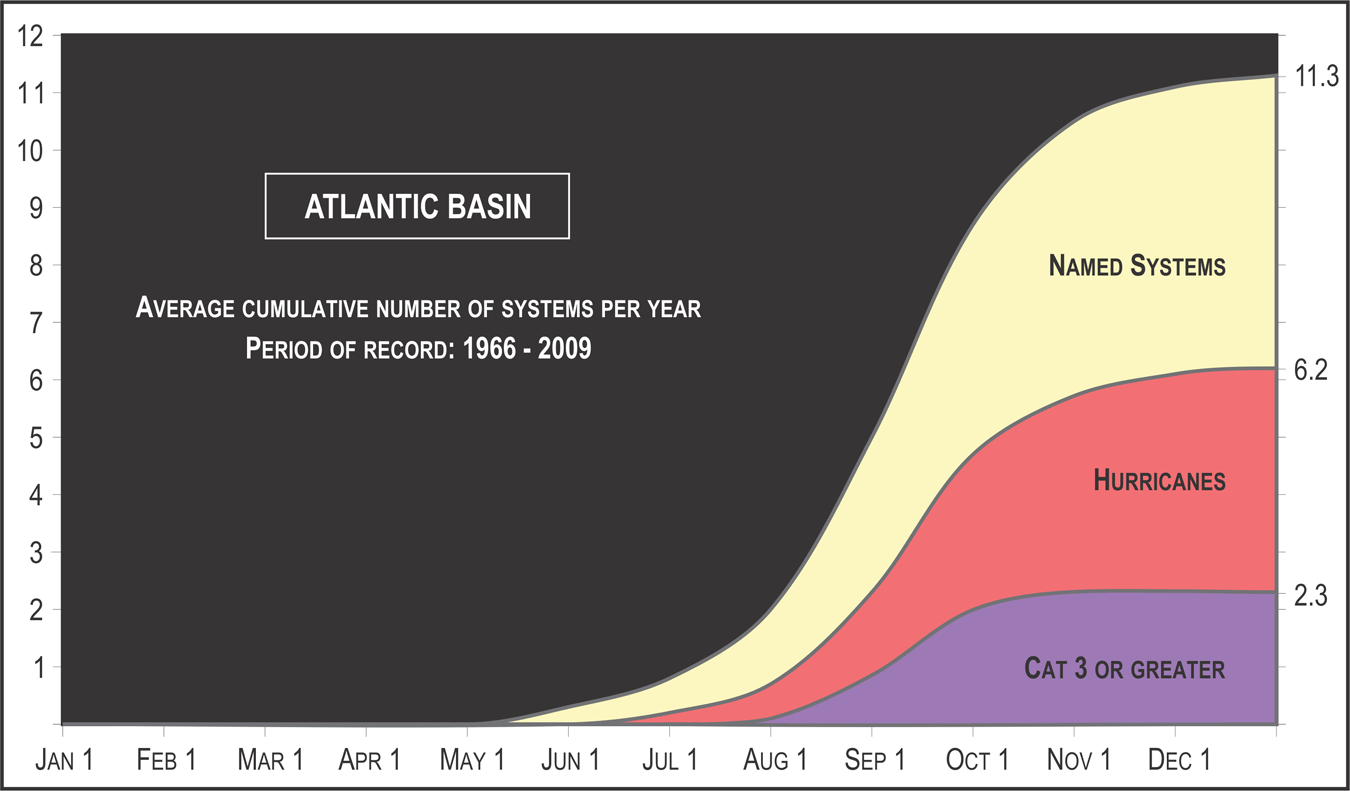
\includegraphics[width=0.5\textwidth]{img/cum-average-cat.png}
\label{fig:cat-climatology}
\end{figure}

\begingroup
\setlength{\tabcolsep}{10pt} % Default value: 6pt
\renewcommand{\arraystretch}{1.5} % Default value: 1
\begin{table}[hbt!]
\centering
\begin{tabular}{|c|c|c|c|c|}
\cline{1-2} \cline{4-5}
\multicolumn{2}{|c|}{\textbf{Tropical Cyclones}} &  & \multicolumn{2}{c|}{\textbf{Other tropical low pressure systems}} \\ \cline{1-2} \cline{4-5} 
category     & wind speed {[}m/s{]}     &  & name                & wind speed {[}m/s{]}               \\ \cline{1-2} \cline{4-5} 
1 & 33--42    &  & tropical depression & $\leq$ 17 \\
2 & 43--49    &  & tropical storm      & 18--32    \\
3 & 50--58    &  &                     &           \\
4 & 58--70    &  &                     &           \\
5 & $\geq$ 70 &  &                     &           \\ \cline{1-2} \cline{4-5} 
\end{tabular}
\caption{Simpson scale defined by 1-minute maximum sustained winds}
\label{tab:simpson-scale}
\end{table}
\endgroup

\begin{enumerate}
\item DONE Classification between tc, tornado, tropical depression...
\item Mention climatology and categorisation
\item Genesis criteria
\item Carnot Cycle
\item Shortly mentioning WISHE Paradigm
\item Mention 1 or 2 of Heini Wernlis Publications
\item use emanuel review paper and cloud dynamics course material
\end{enumerate}


\section{Previous work on TC Tracking}\label{sec:tracking}
\begin{enumerate}
\item Mention work of Christoph Raible/Raibler from Bern regarding TC Tracking
\item See what Heini Wernli has done
\end{enumerate}